% !TeX root = ../main.tex

% Overview
% Explain the system overview
% Design goals
% Explain the system workflow
% Identify system components and explain their function
\chapter{Overview}\label{chapter:overview}
This chapter provides a clear overview of our project, outlining its progress, design goals, and critical components.
We will begin by discussing the shifts in direction that the project has taken due to our new insights.
This reflection was essential as we have noticed that our first assumption was erroneous.
Next, we will discuss the design goals for extending the verifier.
Following this, we will give an overview of how the whole verifier and reproducer combination works and how individual components function.

\section{Course of the Project}
We started this project by evaluating the accuracy and reliability of various emulators.
This entailed researching common emulator bugs and recreating them.
Our main targets were \ac{QEMU} and Arancini, and most of our research was on them.

Our part in this project was focused on developing a program that could produce tests by utilizing symbolic execution on erroneous programs.
Initially, we assumed that a significant proportion of the flaws and inconsistencies discovered in \ac{QEMU} could be attributed to issues within the \ac{TCG}.

Specifically, we suspected that these bugs were caused by erroneous execution paths that led to incorrect jumps within the code. To address this, we planned to use symbolic execution to construct a tree.
This tree was intended to serve as a map, guiding us through the execution path and, therefore, identifying these incorrect jumps.

Through this method, we had hoped to:
\begin{enumerate}[label=(\Alph*)]
   \item Find the shortest path to the error
   \item Recreate the erroneous program by changing the inputs and making sure that it follows the aforementioned path
\end{enumerate}

We wanted to automate test generation and simplify finding emulator bugs through this method.
However, we noticed that most of the bugs stemming from \ac{TCG} were not because of incorrect jumps; they were caused by wrong implementation of instructions.
Because of these findings, our project had a slight change of direction.

Because of our new findings, we stopped concentrating on following the erroneous path and instead concentrated on the offending instructions.
Considering that most of the hard-to-find bugs stem not from the general functionality but the edge cases, we understood that we needed to recreate the state where this bug occurs.
This meant we needed to sample the memory and registers before the erroneous instructions.
We used symbolic execution to find the offending instructions and then leveraged concrete execution to find the actual values.
Combining these two techniques and other code stubs used for running code, we created a tiny executable that could cause the same bug.

\section{Design Goals}
Our main design goal for the reproducer was to extract bugs in the most straightforward manner possible.
This meant the reproducer should need only minimal data, and the resulting program should be as simple as possible.
We hoped to replicate the bugs by utilizing only the provided symbolic traces and concrete values.

We also tried abstracting the detected bug's environment from the required assembly instructions.
This meant we tried to design the reproducer to produce parts of the environment, such as the stack, registers, or memory layout, without necessarily turning them into assembly instructions.
We made this information as flexible as possible to facilitate a more straightforward analysis.

\section{System Workflow and Component's Functions}
The reproducer is designed as an add-on to the Focaccia.
Much of its functionality relies on this verifier.
As shown in the figure \ref{fig:ver_and_rep_1} all the inputs for the reproducer come from it.

\begin{figure}[ht]
   \centering
   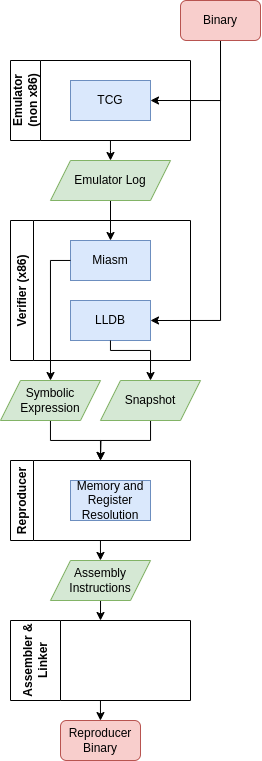
\includegraphics[width=0.45\linewidth]{figures/ver_and_rep_1}
   \caption[verifier and reproducer]{Example flow of the verifier and the reproducer with QEMU}
   \label{fig:ver_and_rep_1}
\end{figure}

\subsection{Inputs}
Both the verifier and the reproducer depend on the same two inputs, namely the emulator log and the binary.
However, there are some peculiarities for both of them.
Any emulator log can be used, regardless of the format, as long as it contains the necessary information.
These logs should either document every change in memory and register values based on the \ac{PC} or provide complete snapshots of memory and register states at each PC.
These are necessary as Focaccia relies on these logs to replicate the emulator's actions accurately.

Another important point about the emulator log is whether it comes from statically linked binaries or dynamically linked binaries.
They need to come from statically linked binaries, which ensures that the program runs with the same set of instructions regardless of the environment in which it is executed.
For instance, discrepancies in the \ac{clib}, whether due to different libraries or versions, can lead to varied instructions.
Such variations would cause the traces not to align, resulting in a trace output filled with errors unrelated to the faulty instruction.

\subsection{First Component: Focaccia the Verifier}

Focaccia is the verifier we use to detect errors in the emulators.
It functions by comparing the change of states in an emulator with that of an oracle.
This oracle is the binary running on its own original \ac{ISA}.
It uses the Miasm reverse engineering framework and the LLDB debugger from LLVM. 
Two inputs are required for the verification: the emulator log and the binary.
Firstly, Focaccia analyzes the instructions in the binary to generate a symbolic trace.
This trace maps out all modifications in memory, registers, and branches.
However, this symbolic trace is not sufficient on its own. 
The binary also provides concrete values from which Focaccia takes snapshots.
Later, these transformations are compared with the emulator log.
If any mismatch is detected, the verifier alerts the users about a bug.

\subsection{Second Component: the Reproducer}
The reproducer add-on's role is to prepare the assembly instructions for triggering a specific bug. 
If enabled by the verifier, it will be run after the verification process is done and the erroneous instructions are found.
The verifier passes the collected snapshot and the symbolic expressions to the reproducer.
The reproducer will use the symbolic expressions to determine which values are needed to trigger this bug and extract these values from the snapshot.
The data flow is depicted in figure \ref{fig:ver_and_rep_1}.
After the memory and register values are determined, they will be combined with the erroneous instruction and other code stubs to produce an assembly program that can be executed.
Ultimately, the reproducer should make debugging easier by recreating an environment similar to the one that caused the original bug.






